\subsection{File Allocation Methods}\label{subsec:File_Allocation_Methods}
The direct-access nature of disks gives us flexibility in the implementation of files.
In almost every case, many files are stored on the same disk.
The main problem is how to allocate space to these files so that disk space is utilized effectively while allowing for quick access to files.

\subsubsection{Contiguous File Allocation}\label{subsubsec:Contiguous_File_Allocation}
Contiguous allocation requires that each file occupy a set of contiguous blocks on the disk.
Disk addresses define a linear ordering on the disk.

Contiguous allocation of a file is defined by the disk address of the first block and length (in blocks).
If the file is $n$ blocks long and starts at location $b$, then it occupies blocks $b, b+1, \ldots, b+n-1$.
The directory entry for each file indicates the address of the starting block and the length of the area allocated for this file.

\paragraph{Advantages of Contiguous Allocation}\label{par:Contiguous_File_Allocation_Advantages}
Accessing a file that has been allocated contiguously is easy.
\begin{itemize}[noitemsep]
\item \textbf{\nameref{subsubsec:Sequential_Access}}.
  \nameref{def:File_System} remembers the disk address of the last block referenced and reads the next block.
\item \textbf{\nameref{subsubsec:Direct_Access}} to block $i$ of a file that starts at block $b$, we can immediately access block $b + i$.
\end{itemize}

\paragraph{Disadvantages of Contiguous Allocation}\label{par:Contiguous_File_Allocation_Disadvantages}
However, this allocation methods has some problems.
One difficulty is finding space for a new file.
The system chosen to manage free space determines how this task is accomplished.
This is another case of the \nameref{def:Allocation_Problem}.

\begin{definition}[Allocation Problem]\label{def:Allocation_Problem}
  The \emph{Allocation Problem} involves how to satisfy a request of size $n$ from a list of free holes.
  If the holes are not organized, i.e.\ there are enough blocks but they are not contiguous, then the request cannot be serviced.
\end{definition}

\nameref{subpar:First_Fit} and \nameref{subpar:Best_Fit} are the most common strategies used to select a free hole from the set of available holes, however, \nameref{subpar:Worst_Fit} is also possible.
Simulations have shown that both first fit and best fit are more efficient than worst fit in terms of time and storage utilization.
However, \textbf{all these algorithms} suffer from the problem of \nameref{def:External_Fragmentation}.
As files are allocated and deleted, the free disk space is broken into little pieces.
External fragmentation exists whenever free space is broken into chunks.
Fixing this problem is only solvable by garbage collection, in this case means moving all data to another disk then copying it back.

Another problem is determining how much space is needed for a file.
When the file is created, the total amount of space it will need must be found and allocated.
\begin{itemize}[noitemsep]
\item If we allocate too little space to a file, we may find that the file cannot be extended.
\item If the total amount of space needed for a file is known in advance, preallocation may be inefficient.
\end{itemize}

To minimize these drawbacks, some operating systems use a modified contiguous-allocation scheme.
Here, a contiguous chunk of space is allocated initially.
Then, if that amount proves not to be large enough, another chunk of contiguous space, known as an \nameref{def:Extent}, is added.
The location of a file’s blocks is then recorded as a location and a block count, plus a link to the first block of the next extent.

\begin{definition}[Extent]\label{def:Extent}
  An \emph{extent} is used in a \nameref{subsubsec:Contiguous_File_Allocation} scheme, and is just another contiguous block(s) of storage that has been given to a file for use.
  Extents are allocated on an as-needed basis.
\end{definition}

\subsubsection{Linked File Allocation}\label{subsubsec:Linked_File_Allocation}
Linked allocation solves all problems of \nameref{subsubsec:Contiguous_File_Allocation} (\Cref{par:Contiguous_File_Allocation_Disadvantages}).
With linked allocation, each \nameref{def:File} is a linked list of disk blocks; the disk blocks may be scattered anywhere on the disk.
The \nameref{def:Directory} contains a pointer to the first and last blocks of each file entry.
Each block contains a pointer to the next block.
These pointers are not made available to the user.
Thus, if each block is 512 bytes in size, and a disk address (the pointer) requires 4 bytes, then the user sees blocks of 508 bytes.

To create a new \nameref{def:File}, we simply create a new entry in the \nameref{def:Directory}.
With linked allocation, each directory entry has a pointer to the first disk block of the file, which is initialized to \texttt{null} (or the end-of-list pointer value), signifying an empty file.
The size field is also set to 0.
A subsequent \kernelinline{write()} to the file causes the free-space management system to find a free block, write to this new block, and link it to the end of the file.
To read a file, we simply read blocks by following the pointers from block to block.

\paragraph{Advantages of Linked Allocation}\label{par:Linked_File_Allocation_Advantages}
There is no \nameref{def:External_Fragmentation} with linked allocation, and any free block on the free-space list can be used to satisfy a request.
However, minor \nameref{def:Internal_Fragmentation} can occur when a file's last block is only partly used; but there is little that can be done about that.

The size of a file need not be declared when the file is created.
A file can continue to grow as long as free blocks are available.
Consequently, it is never necessary to compact disk space.

\paragraph{Disadvantages of Linked Allocation}\label{par:Linked_File_Allocation_Disadvantages}
The major problem is that it can be used effectively only for \nameref{subsubsec:Sequential_Access} files.
To find the $i$th block of a file, we must start at the beginning of that file and follow the pointers until we get to the ith block.
Each access to a pointer requires a disk read, and some require a disk seek.
Consequently, it is inefficient to support a \nameref{subsubsec:Direct_Access} capability for linked-allocation files.

Another disadvantage is the space required for the pointers.
If a pointer requires 4 bytes out of a 512-byte block, then \SI{0.78}{\percent} percent of the disk is being used for pointers, rather than for information.
Thus, each file requires slightly more blocks than it would otherwise.
The usual solution to this problem is to collect blocks into multiples, called \nameref{def:Disk_Cluster}s, and to allocate clusters rather than blocks.
For instance, the file system may define a cluster as four blocks and operate on the disk only in cluster units.
Then, the pointers use a much smaller percentage of the file’s disk space.

\begin{definition}[Cluster]\label{def:Disk_Cluster}
  A \emph{cluster} is a collection of blocks used in a \nameref{subsubsec:Linked_File_Allocation} scheme.
  Using a cluster in this scheme allows for more data to be addressed by a single pointer in the cluster.
  Meaning, the average utilization of the disk to other cluster pointers is minimized.
\end{definition}

Using \nameref{def:Disk_Cluster}s has the cost of increasing \nameref{def:Internal_Fragmentation}, because more space is wasted when a cluster is partially full than when a block is partially full.
Clusters can be used to improve the disk-access time for many other algorithms as well, so they are used in most file systems.

Another problem of linked allocation is reliability.
Since files are linked together by pointers scattered all over the disk, consider what would happen if just a single file pointer were lost or damaged.
A bug in the operating-system software or a disk hardware failure might result in picking up the wrong pointer.
This error could in turn result in linking into the free-space list or into another file.

Some partial solutions are:
\begin{itemize}[noitemsep]
\item Use doubly linked lists
\item Store the file name and relative block number in each block.
\end{itemize}
However, these solutions require even more overhead for each file.

\paragraph{File-Allocation Table}\label{par:File_Allocation_Table}
File-Allocation Table (FAT) is a simple and efficient method of disk-space allocation that was used by the \textsc{ms-dos} operating system.
FAT is still commonly used today in external flash media, like flash drives.

In this system, there are 3 major disk components:
\begin{enumerate}[noitemsep]
\item The Directory.
  \begin{itemize}[noitemsep]
  \item Contains one entry for every \nameref{def:File} in that directory, including subdirectories.
  \item Stores the name and the starting block of the file.
  \item May contain additional information about the file here too.
  \end{itemize}
\item The File Allocation Table itself.
  \begin{itemize}[noitemsep]
  \item There is one entry in this table for \textbf{EACH} data block on this disk's \nameref{def:File_System}.
  \item The index of each entry corresponds to that same numbered block in the data blocks.
  \item Each entry here \textbf{MAY} also contain a pointer to the next data block this file inhabits.
    \begin{itemize}[noitemsep]
    \item The maximum size of this pointer determines how big the biggest file may be.
    \item In the original FAT, this pointer was 12 bytes.
    \item In the more common FAT32, this pointer is 32 bytes, making the largest possible single file \SI{4}{\gibi{} \byte{}}.
    \end{itemize}
  \item The existence of this block in this chain means this file \textbf{USES} these data blocks.
  \item This table is small enough to be cached in memory for quick file lookups.
  \end{itemize}
\item The Data blocks.
  \begin{itemize}[noitemsep]
  \item These are just the data blocks.
  \item They are not cached in any way.
  \item They are fetched when the \nameref{def:Operating_System} traverses the FAT.\@
  \end{itemize}
\end{enumerate}

The use of the File Allocation Table to find a set of blocks on-disk is shown in \Cref{fig:File_Allocation_Table}.
\begin{figure}[h!tbp]
  \centering
  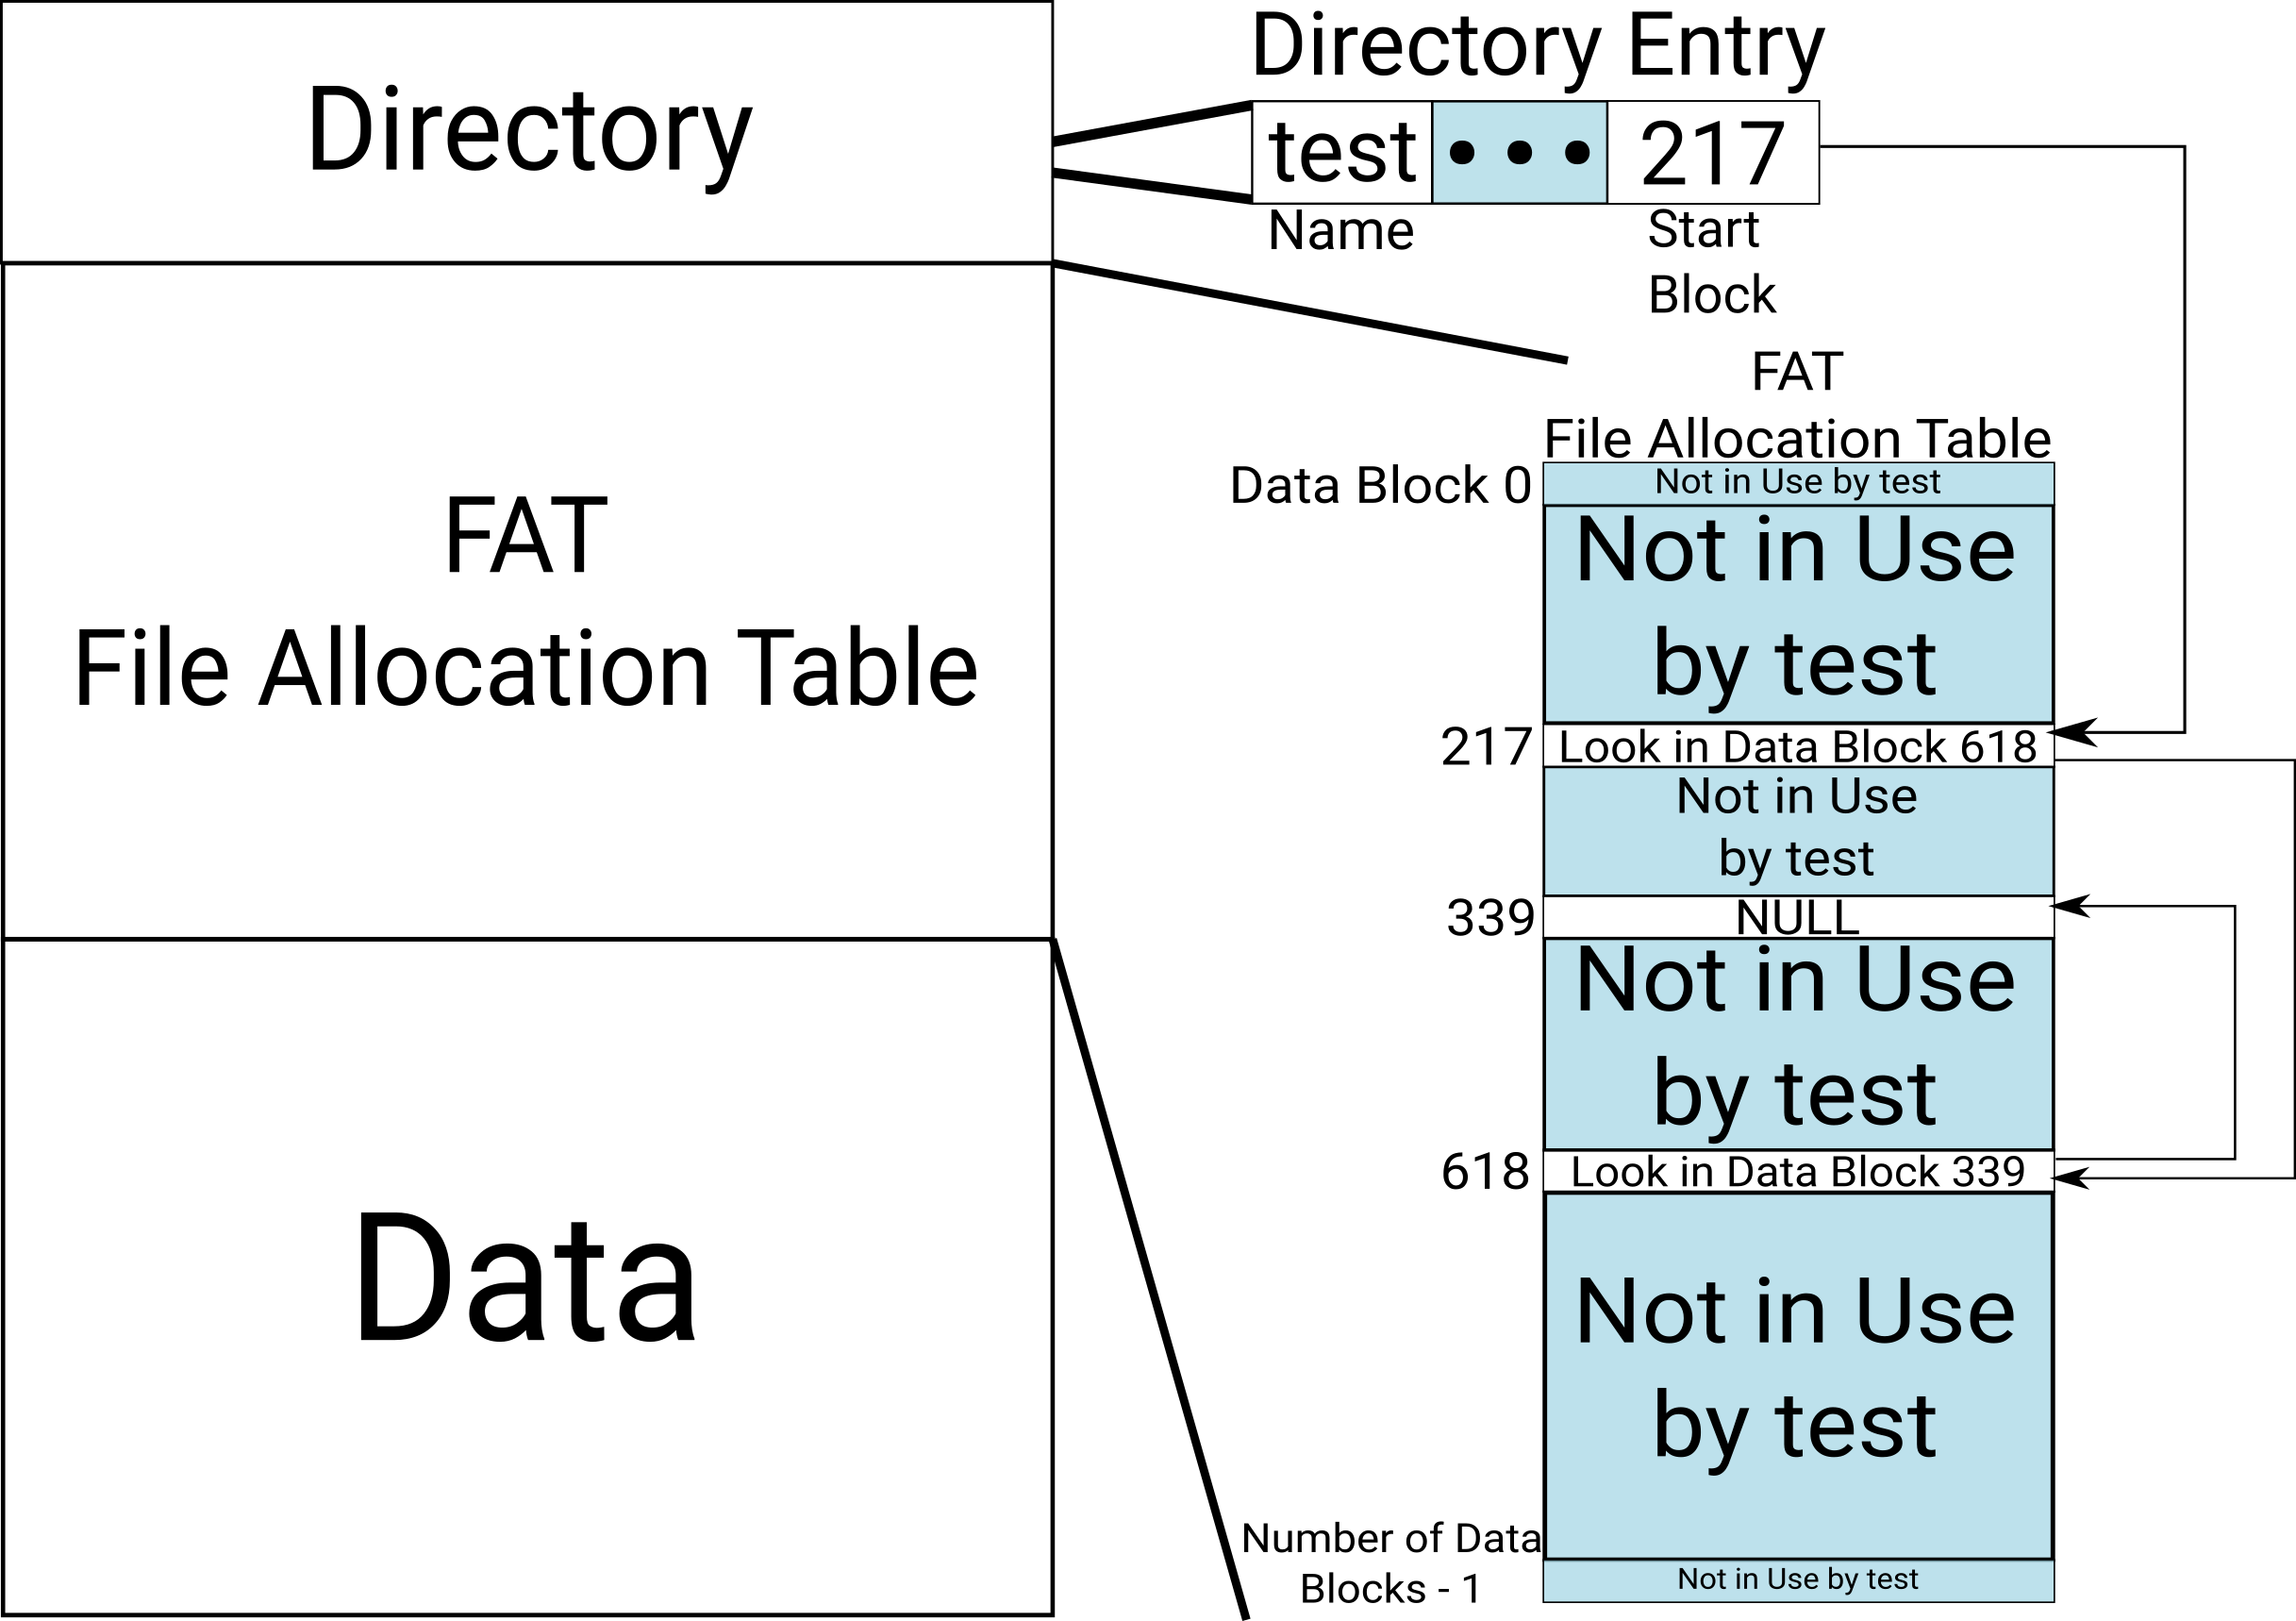
\includegraphics[scale=0.9]{./Drawings/EDAF35-Operating_Systems/FAT.png}
  \caption{File Allocation Table}
  \label{fig:File_Allocation_Table}
\end{figure}

\subsubsection{Indexed File Allocation}\label{subsubsec:Indexed_File_Allocation}
Indexed allocation solves the problem of pure \nameref{subsubsec:Linked_File_Allocation} by bringing all the pointers together into one location: the index block.
In the absence of a \nameref{par:File_Allocation_Table}, linked allocation cannot support efficient direct access.
The pointers to the blocks are scattered with the blocks themselves all over the disk and must be retrieved in order.
Linked allocation solves the \nameref{def:External_Fragmentation} and size-declaration problems of \nameref{subsubsec:Contiguous_File_Allocation}.

Each file has its own index block, which is an array of disk-block addresses.
The $i$th entry in the index block points to the $i$th block of the file.
The directory contains the address of the index block.
To find and read the $i$th block, we use the pointer in the $i$th index-block entry.
This is similar to the \nameref{def:Paging} scheme discussed in \Cref{subsec:Paging}.

When the file is created, all pointers in the index block are set to \texttt{null}.
When the $i$th block is first written, a block is obtained from the free-space manager, and its address is put in the $i$th index-block entry.

\paragraph{Advantages of Indexed Allocation}\label{par:Indexed_File_Allocation_Advantages}
Indexed allocation supports direct access, without suffering from \nameref{def:External_Fragmentation}, because any free block on the disk can satisfy a request for more space.

\paragraph{Disadvantages of Indexed Allocation}\label{par:Indexed_File_Allocation_Disadvantages}
Indexed-allocation schemes suffer from some of the same performance problems as does linked allocation.
Specifically, the index blocks can be cached in memory, but the data blocks may be spread all over a volume.

Indexed allocation does still suffer from wasted space.
The pointer overhead of the index block is generally greater than the pointer overhead of linked allocation.
This is especially true when a file requires fewer blocks than an index block can address.
This raises the question of how large the index block should be.
Every file must have an index block, so we want the index block to be as small as possible.
If the index block is \textbf{too} small, it will not be able to hold enough pointers for a large file.

To handle this, there are 3 common mechanisms:
\begin{enumerate}[noitemsep]
\item \textbf{Linked scheme}.
  \begin{itemize}[noitemsep]
  \item An index block is normally one disk block.
    Thus, it can be read and written directly itself.
  \item To allow for large files, link together several index blocks.
  \item The last address-sized hole in the index block is \texttt{null} for small files, or is a pointer to another index block, for a large file.
\end{itemize}

\item \textbf{Multilevel index}.
  A variant of linked representation uses a first-level index
block to point to a set of second-level index blocks, which in turn point to
the file blocks. To access a block, the operating system uses the first-level
index to find a second-level index block and then uses that block to find the
desired data block. This approach could be continued to a third or fourth
level, depending on the desired maximum file size.

\item \textbf{Combined scheme}.
  This forms the basis of a \textsc{unix} \nameref{par:Inode}.
\end{enumerate}

\paragraph{\textsc{unix} \texttt{inode}}\label{par:Inode}
The \texttt{inode} is used in \textsc{unix}-based file systems.
The \texttt{inode} keeps the first 15 pointers of the index block in the \texttt{inode}.
\begin{itemize}[noitemsep]
\item The \texttt{inode} does contain a little bit of data within itself.
\item The first 12 of these pointers point directly to data blocks (they contain addresses of blocks that contain data of the file).
  Thus, the data for small files does not need a separate index block.
\item The 13th points to a single indirect block.
  \begin{itemize}[noitemsep]
  \item This is an index block containing the addresses of blocks that contain data.
  \item The redirection index block (the one from dereferencing the single indirect in the \texttt{inode}) can have as many pointer to data blocks as a block allows.
\end{itemize}

\item The 14th points to a double indirect block, which contains the address of a block that contains the addresses of blocks that contain pointers to the actual data blocks.
  \begin{itemize}[noitemsep]
  \item Each of the redirection index blocks (the one from dereferencing an indirection) can have as many pointer to data blocks as a block allows.
  \end{itemize}
\item The last pointer contains the address of a triple indirect block.
  \begin{itemize}[noitemsep]
  \item Like the other indirect blocks, it must be dereferenced multiple times to get to the actual data.
  \item Each of the redirection index blocks (the one from dereferencing an indirection) can have as many pointer to data blocks as a block allows.
  \end{itemize}
\end{itemize}

A visualization of the \textsc{unix} \texttt{inode} is shown in \Cref{fig:Inode}.

\begin{figure}[h!tbp]
  \centering
  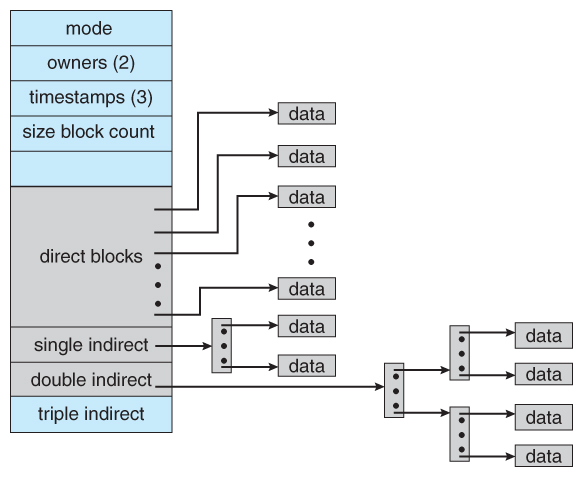
\includegraphics[scale=1.0]{./Drawings/EDAF35-Operating_Systems/UNIX_inode.jpg}
  \caption{\textsc{unix} \texttt{inode}}
  \label{fig:Inode}
\end{figure}


%%% Local Variables:
%%% mode: latex
%%% TeX-master: "../../EDAF35-Operating_Systems-Reference_Sheet"
%%% End:
